%% bare_jrnl.tex
%% V1.3
%% 2007/01/11
%% by Michael Shell
%% see http://www.michaelshell.org/
%% for current contact information.
%%
%% This is a skeleton file demonstrating the use of IEEEtran.cls
%% (requires IEEEtran.cls version 1.7 or later) with an IEEE journal paper.
%%
%% Support sites:
%% http://www.michaelshell.org/tex/ieeetran/
%% http://www.ctan.org/tex-archive/macros/latex/contrib/IEEEtran/
%% and
%% http://www.ieee.org/




\documentclass[journal]{IEEEtran}
\usepackage{blindtext}
\usepackage{graphicx}


% *** CITATION PACKAGES ***
%
\usepackage{cite}

% *** GRAPHICS RELATED PACKAGES ***
%
\ifCLASSINFOpdf
  % \usepackage[pdftex]{graphicx}
  % declare the path(s) where your graphic files are
  % \graphicspath{{../pdf/}{../jpeg/}}
  % and their extensions so you won't have to specify these with
  % every instance of \includegraphics
  % \DeclareGraphicsExtensions{.pdf,.jpeg,.png}
\else
  % or other class option (dvipsone, dvipdf, if not using dvips). graphicx
  % will default to the driver specified in the system graphics.cfg if no
  % driver is specified.
  % \usepackage[dvips]{graphicx}
  % declare the path(s) where your graphic files are
  % \graphicspath{{../eps/}}
  % and their extensions so you won't have to specify these with
  % every instance of \includegraphics
  % \DeclareGraphicsExtensions{.eps}
\fi
% graphicx was written by David Carlisle and Sebastian Rahtz. It is
% required if you want graphics, photos, etc. graphicx.sty is already
% installed on most LaTeX systems. The latest version and documentation can
% be obtained at: 
% http://www.ctan.org/tex-archive/macros/latex/required/graphics/
% Another good source of documentation is "Using Imported Graphics in
% LaTeX2e" by Keith Reckdahl which can be found as epslatex.ps or
% epslatex.pdf at: http://www.ctan.org/tex-archive/info/
%
% latex, and pdflatex in dvi mode, support graphics in encapsulated
% postscript (.eps) format. pdflatex in pdf mode supports graphics
% in .pdf, .jpeg, .png and .mps (metapost) formats. Users should ensure
% that all non-photo figures use a vector format (.eps, .pdf, .mps) and
% not a bitmapped formats (.jpeg, .png). IEEE frowns on bitmapped formats
% which can result in "jaggedy"/blurry rendering of lines and letters as
% well as large increases in file sizes.
%
% You can find documentation about the pdfTeX application at:
% http://www.tug.org/applications/pdftex





% *** MATH PACKAGES ***
%
%\usepackage[cmex10]{amsmath}
% A popular package from the American Mathematical Society that provides
% many useful and powerful commands for dealing with mathematics. If using
% it, be sure to load this package with the cmex10 option to ensure that
% only type 1 fonts will utilized at all point sizes. Without this option,
% it is possible that some math symbols, particularly those within
% footnotes, will be rendered in bitmap form which will result in a
% document that can not be IEEE Xplore compliant!
%
% Also, note that the amsmath package sets \interdisplaylinepenalty to 10000
% thus preventing page breaks from occurring within multiline equations. Use:
%\interdisplaylinepenalty=2500
% after loading amsmath to restore such page breaks as IEEEtran.cls normally
% does. amsmath.sty is already installed on most LaTeX systems. The latest
% version and documentation can be obtained at:
% http://www.ctan.org/tex-archive/macros/latex/required/amslatex/math/





% *** SPECIALIZED LIST PACKAGES ***
%
%\usepackage{algorithmic}
% algorithmic.sty was written by Peter Williams and Rogerio Brito.
% This package provides an algorithmic environment fo describing algorithms.
% You can use the algorithmic environment in-text or within a figure
% environment to provide for a floating algorithm. Do NOT use the algorithm
% floating environment provided by algorithm.sty (by the same authors) or
% algorithm2e.sty (by Christophe Fiorio) as IEEE does not use dedicated
% algorithm float types and packages that provide these will not provide
% correct IEEE style captions. The latest version and documentation of
% algorithmic.sty can be obtained at:
% http://www.ctan.org/tex-archive/macros/latex/contrib/algorithms/
% There is also a support site at:
% http://algorithms.berlios.de/index.html
% Also of interest may be the (relatively newer and more customizable)
% algorithmicx.sty package by Szasz Janos:
% http://www.ctan.org/tex-archive/macros/latex/contrib/algorithmicx/




% *** ALIGNMENT PACKAGES ***
%
\usepackage{array}
% Frank Mittelbach's and David Carlisle's array.sty patches and improves
% the standard LaTeX2e array and tabular environments to provide better
% appearance and additional user controls. As the default LaTeX2e table
% generation code is lacking to the point of almost being broken with
% respect to the quality of the end results, all users are strongly
% advised to use an enhanced (at the very least that provided by array.sty)
% set of table tools. array.sty is already installed on most systems. The
% latest version and documentation can be obtained at:
% http://www.ctan.org/tex-archive/macros/latex/required/tools/


\usepackage{mdwmath}
\usepackage{mdwtab}
% Also highly recommended is Mark Wooding's extremely powerful MDW tools,
% especially mdwmath.sty and mdwtab.sty which are used to format equations
% and tables, respectively. The MDWtools set is already installed on most
% LaTeX systems. The lastest version and documentation is available at:
% http://www.ctan.org/tex-archive/macros/latex/contrib/mdwtools/


% IEEEtran contains the IEEEeqnarray family of commands that can be used to
% generate multiline equations as well as matrices, tables, etc., of high
% quality.


%\usepackage{eqparbox}
% Also of notable interest is Scott Pakin's eqparbox package for creating
% (automatically sized) equal width boxes - aka "natural width parboxes".
% Available at:
% http://www.ctan.org/tex-archive/macros/latex/contrib/eqparbox/

\usepackage[justification=centering]{caption}





% *** SUBFIGURE PACKAGES ***
\usepackage[tight,footnotesize]{subfigure}
% subfigure.sty was written by Steven Douglas Cochran. This package makes it
% easy to put subfigures in your figures. e.g., "Figure 1a and 1b". For IEEE
% work, it is a good idea to load it with the tight package option to reduce
% the amount of white space around the subfigures. subfigure.sty is already
% installed on most LaTeX systems. The latest version and documentation can
% be obtained at:
% http://www.ctan.org/tex-archive/obsolete/macros/latex/contrib/subfigure/
% subfigure.sty has been superceeded by subfig.sty.



%\usepackage[caption=false]{caption}
%\usepackage[font=footnotesize]{subfig}
% subfig.sty, also written by Steven Douglas Cochran, is the modern
% replacement for subfigure.sty. However, subfig.sty requires and
% automatically loads Axel Sommerfeldt's caption.sty which will override
% IEEEtran.cls handling of captions and this will result in nonIEEE style
% figure/table captions. To prevent this problem, be sure and preload
% caption.sty with its "caption=false" package option. This is will preserve
% IEEEtran.cls handing of captions. Version 1.3 (2005/06/28) and later 
% (recommended due to many improvements over 1.2) of subfig.sty supports
% the caption=false option directly:
%\usepackage[caption=false,font=footnotesize]{subfig}
%
% The latest version and documentation can be obtained at:
% http://www.ctan.org/tex-archive/macros/latex/contrib/subfig/
% The latest version and documentation of caption.sty can be obtained at:
% http://www.ctan.org/tex-archive/macros/latex/contrib/caption/




% *** FLOAT PACKAGES ***
%
%\usepackage{fixltx2e}
% fixltx2e, the successor to the earlier fix2col.sty, was written by
% Frank Mittelbach and David Carlisle. This package corrects a few problems
% in the LaTeX2e kernel, the most notable of which is that in current
% LaTeX2e releases, the ordering of single and double column floats is not
% guaranteed to be preserved. Thus, an unpatched LaTeX2e can allow a
% single column figure to be placed prior to an earlier double column
% figure. The latest version and documentation can be found at:
% http://www.ctan.org/tex-archive/macros/latex/base/


%\usepackage{stfloats}
% stfloats.sty was written by Sigitas Tolusis. This package gives LaTeX2e
% the ability to do double column floats at the bottom of the page as well
% as the top. (e.g., "\begin{figure*}[!b]" is not normally possible in
% LaTeX2e). It also provides a command:
%\fnbelowfloat
% to enable the placement of footnotes below bottom floats (the standard
% LaTeX2e kernel puts them above bottom floats). This is an invasive package
% which rewrites many portions of the LaTeX2e float routines. It may not work
% with other packages that modify the LaTeX2e float routines. The latest
% version and documentation can be obtained at:
% http://www.ctan.org/tex-archive/macros/latex/contrib/sttools/
% Documentation is contained in the stfloats.sty comments as well as in the
% presfull.pdf file. Do not use the stfloats baselinefloat ability as IEEE
% does not allow \baselineskip to stretch. Authors submitting work to the
% IEEE should note that IEEE rarely uses double column equations and
% that authors should try to avoid such use. Do not be tempted to use the
% cuted.sty or midfloat.sty packages (also by Sigitas Tolusis) as IEEE does
% not format its papers in such ways.


%\ifCLASSOPTIONcaptionsoff
%  \usepackage[nomarkers]{endfloat}
% \let\MYoriglatexcaption\caption
% \renewcommand{\caption}[2][\relax]{\MYoriglatexcaption[#2]{#2}}
%\fi
% endfloat.sty was written by James Darrell McCauley and Jeff Goldberg.
% This package may be useful when used in conjunction with IEEEtran.cls'
% captionsoff option. Some IEEE journals/societies require that submissions
% have lists of figures/tables at the end of the paper and that
% figures/tables without any captions are placed on a page by themselves at
% the end of the document. If needed, the draftcls IEEEtran class option or
% \CLASSINPUTbaselinestretch interface can be used to increase the line
% spacing as well. Be sure and use the nomarkers option of endfloat to
% prevent endfloat from "marking" where the figures would have been placed
% in the text. The two hack lines of code above are a slight modification of
% that suggested by in the endfloat docs (section 8.3.1) to ensure that
% the full captions always appear in the list of figures/tables - even if
% the user used the short optional argument of \caption[]{}.
% IEEE papers do not typically make use of \caption[]'s optional argument,
% so this should not be an issue. A similar trick can be used to disable
% captions of packages such as subfig.sty that lack options to turn off
% the subcaptions:
% For subfig.sty:
% \let\MYorigsubfloat\subfloat
% \renewcommand{\subfloat}[2][\relax]{\MYorigsubfloat[]{#2}}
% For subfigure.sty:
% \let\MYorigsubfigure\subfigure
% \renewcommand{\subfigure}[2][\relax]{\MYorigsubfigure[]{#2}}
% However, the above trick will not work if both optional arguments of
% the \subfloat/subfig command are used. Furthermore, there needs to be a
% description of each subfigure *somewhere* and endfloat does not add
% subfigure captions to its list of figures. Thus, the best approach is to
% avoid the use of subfigure captions (many IEEE journals avoid them anyway)
% and instead reference/explain all the subfigures within the main caption.
% The latest version of endfloat.sty and its documentation can obtained at:
% http://www.ctan.org/tex-archive/macros/latex/contrib/endfloat/
%
% The IEEEtran \ifCLASSOPTIONcaptionsoff conditional can also be used
% later in the document, say, to conditionally put the References on a 
% page by themselves.





% *** PDF, URL AND HYPERLINK PACKAGES ***
%
\usepackage{url}
% url.sty was written by Donald Arseneau. It provides better support for
% handling and breaking URLs. url.sty is already installed on most LaTeX
% systems. The latest version can be obtained at:
% http://www.ctan.org/tex-archive/macros/latex/contrib/misc/
% Read the url.sty source comments for usage information. Basically,
% \url{my_url_here}.





% *** Do not adjust lengths that control margins, column widths, etc. ***
% *** Do not use packages that alter fonts (such as pslatex).         ***
% There should be no need to do such things with IEEEtran.cls V1.6 and later.
% (Unless specifically asked to do so by the journal or conference you plan
% to submit to, of course. )


% correct bad hyphenation here
\hyphenation{op-tical net-works semi-conduc-tor}


\begin{document}
%
% paper title
% can use linebreaks \\ within to get better formatting as desired
\title{Hybrid Multi-Robot Coordination in Smart Factory Warehouses}
%
%
% author names and IEEE memberships
% note positions of commas and nonbreaking spaces ( ~ ) LaTeX will not break
% a structure at a ~ so this keeps an author's name from being broken across
% two lines.
% use \thanks{} to gain access to the first footnote area
% a separate \thanks must be used for each paragraph as LaTeX2e's \thanks
% was not built to handle multiple paragraphs
%

%TODO
%Add your names here (alphabetically):

\author{Group 3 - Vincent W\"olfer, Florian Ziesche, Patrick Denzler, Shreyas Gokhale, Uros Petkovic}

% note the % following the last \IEEEmembership and also \thanks - 
% these prevent an unwanted space from occurring between the last author name
% and the end of the author line. i.e., if you had this:
% 
% \author{....lastname \thanks{...} \thanks{...} }
%                     ^------------^------------^----Do not want these spaces!
%
% a space would be appended to the last name and could cause every name on that
% line to be shifted left slightly. This is one of those "LaTeX things". For
% instance, "\textbf{A} \textbf{B}" will typeset as "A B" not "AB". To get
% "AB" then you have to do: "\textbf{A}\textbf{B}"
% \thanks is no different in this regard, so shield the last } of each \thanks
% that ends a line with a % and do not let a space in before the next \thanks.
% Spaces after \IEEEmembership other than the last one are OK (and needed) as
% you are supposed to have spaces between the names. For what it is worth,
% this is a minor point as most people would not even notice if the said evil
% space somehow managed to creep in.



% The paper headers
%\markboth{Journal of \LaTeX\ Class Files,~Vol.~6, No.~1, January~2007}%
%{Shell \MakeLowercase{\textit{et al.}}: Bare Demo of IEEEtran.cls for %Journals}

\markboth{App-Ras: Final Project Report}%
{Application of Robotics and Autonomous Systems}



% The only time the second header will appear is for the odd numbered pages
% after the title page when using the twoside option.
% 
% *** Note that you probably will NOT want to include the author's ***
% *** name in the headers of peer review papers.                   ***
% You can use \ifCLASSOPTIONpeerreview for conditional compilation here if
% you desire.




% If you want to put a publisher's ID mark on the page you can do it like
% this:
%\IEEEpubid{0000--0000/00\$00.00~\copyright~2007 IEEE}
% Remember, if you use this you must call \IEEEpubidadjcol in the second
% column for its text to clear the IEEEpubid mark.



% use for special paper notices
%\IEEEspecialpapernotice{(Invited Paper)}




% make the title area
\maketitle


\begin{abstract}
%\boldmath
You should summarize your work here. A good intro with one sentence: e.g. This technology is needed due to …. Then how you approached to the problem. What is your contribution/the most valuable part of the work emphasis that. What methodologies you used. How you demonstrated your results. How was the system performance. It should not be too short or too long
\end{abstract}
% IEEEtran.cls defaults to using nonbold math in the Abstract.
% This preserves the distinction between vectors and scalars. However,
% if the journal you are submitting to favors bold math in the abstract,
% then you can use LaTeX's standard command \boldmath at the very start
% of the abstract to achieve this. Many IEEE journals frown on math
% in the abstract anyway.

% Note that keywords are not normally used for peerreview papers.
\begin{IEEEkeywords}
IEEEtran, journal, \LaTeX, paper, template.
\end{IEEEkeywords}






% For peer review papers, you can put extra information on the cover
% page as needed:
% \ifCLASSOPTIONpeerreview
% \begin{center} \bfseries EDICS Category: 3-BBND \end{center}
% \fi
%
% For peerreview papers, this IEEEtran command inserts a page break and
% creates the second title. It will be ignored for other modes.
\IEEEpeerreviewmaketitle

\section{Introduction}
\subsection{Motivation}
\label{sec:motivation}
A smart factory environment is an important aspect of "Industry 4.0" where products can be ordered, produced, sorted and stored in a warehouse to be finally delivered to the recipient. The different components of the scenario are modular and hence the information exchange between them is limited.
\\
The goal of our project is to implement a scalable system for cooperative multi-agent task and path planning. The project is used in a warehouse scenario, where robot agents have to store packages into shelves as per the tasks issued. These packages theoretically arrive without any pre-planning and hence the system should be able to accommodate for the unpredictable demand.
\\
To increase efficiency the transportation, multiple robots have to work in parallel in a limited driving space of a warehouse and with co-ordination with the other robots to avoid collisions.
\\
Congestion is another conundrum that this system has to consider. The robots will lose valuable time if they have to wait due to congestion, reducing lower the overall effectiveness of the warehouse system.
\\
This project strives to provide a solution for the problem of assigning packages to the robots, planning the driving paths of the robots and coordinating them. The problem can be split into two separate parts: the task planning and the path planning. Both parts have to incorporate the coordination aspect.
\\
The task planning is concerned with assigning incoming packages to the robots considering the time needed to store the package, energy consumption of the robots and overall optimality as far as possible given that the packages arrive
randomly. The technical challenge here is to find an algorithm can assign a package to the best robot under the previously mentioned considerations.
\\
The path planning is concerned with finding and traversing an optimal path for a robot between two points in the known area of indoor warehouse, with consideration of the other moving robots, non-holonomity criteria for optimality reasons and a continuous, non-linear environment. The technical problem is to find an algorithm which plans an optimal path for a robot under the
previously mentioned considerations.
\\
\subsection{Problem Definition}
A successful implementation of the project will go through following steps:
\begin{itemize}
\item The project starts with receiving a package that is to be stored in the warehouse.
\item The pick-up point on which the package arrives and the drop-off point, where the package is to be stored, together constitute a task that has to be assigned to a robot. An example of such a task would be to place the package from the input tray to the storage tray. 
\item The system should accordingly decide a storage tray and assign the task to a suitable robot agent.
\item The agent should be able to successfully navigate through the environment using the path and task planner and deliver the package. Thus, finishing the task
\item The system must be stable enough to be able to perform multiple tasks concurrently and accommodate for inter-robot interactions.  
\end{itemize} 
\subsection{Related Literature}
how literature approaches to it (very briefly as we have a related works section)

\subsection{Approach}
To approach this problem, we first considered the state of the initial framework which was given. We received a morse-ros project which already included: 
1. A functioning morse environment for indoor warehouse with a demo map 2. ROS environment with essential components, excluding path and task planning. 3. A bridge between ROS and Morse environments.  
\\
The first step was to classify problem into different tasks. The main tasks were Path planning and Task Planning and then we divided them further into subtasks. After literature survey, we decided on top-level system that we will try to implement. For example: using decentralized architecture for path planning with coordination within the robot agents for path reservations. Accordingly we set following objectives to be met:
\begin{itemize}
\item To use existing system as a base architecture  
\item Implementing and testing different path planning algorithms such as RRT* and Theta*-heurisitc in ROS environment
\item Decentralized Multi- Robot collaboration
\item Hybrid (decentralized election but centralized assignment) task planner 
\end{itemize}
In the second step of planning, we started by analysing our top level goal: To successfully implement task and path planning with multi robot collaboration and then setting assigning it for milestone 2. For path planning the research and demo implementation of the algorithm was first step. We compared and demonstrated different path planning approaches such as Theta* and RRT* on a C++ based environment and decided our milestones for implementations on ROS. Another important aspect of our system was Multi-Robot collaboration, which we decided to implement after the second milestone.  A detail working of the system will be explained in \ref{sec:methodology}.
%%MIlestone picture
\\
Finally, we decided to analyse the results based on a number of criterion which we thought might be useful for a warehousing scenario. For example: average time taken for a successful completion of the task and average time spent in different activities by each robot agent. These parameters are indicative of some interesting matrics such as what is the impact of increasing number of robots on the system and how often a robot agent needs charging. More evaluation methods and results will be explained in \ref{sec:results} 

\section{Related Work}
\label{sec:related_work}
%Paste from SDS
%TODO check and improve
%TODO Add references at the right places	
Different algorithms have been developed for path planning. One of the approaches is that we present the space as a potential field, where obstacles have high potential and the goal point has a low potential. Although the computation difficulty is low, the artificial potential fields method did not have much success in more complex environments.
\\
One of the first proposed algorithms was A* [1] which is based on a grid-based search where the robot is allowed to move just on the line between adjacent grid points. Based on the A* algorithm several variants for optimal multi-agent pathfinding were submitted. However, the feebleness of the algorithm is the constraint of moving just between the lines connecting the grid points. This weakness was eliminated with Theta* algorithm [2], where the path is not constrained by edges of adjacent grids.
\\
Probabilistic roadmap (PRM) [3] is a sampling-based approach where the random samples are taken and tested if they fulfil the constraints of the space. Connecting points that are near each other a roadmap is built. The path is estimated by a graph searching algorithm. Comparing to other approaches PRM is slower and takes more computational effort.
\\
In 1998 the rapidly-exploring random trees (RRT) was proposed [4]. Later it was significantly improved with RRT* [5], which is a variant of RRT that converges towards an optimal solution. In recent years it is one of the most used algorithms and there are many variants of RRT* that try to optimize the search of the path. One of them is Theta*-RRT [6] that is two-phase path planner. In the first phase it uses Theta* to estimate the path, which is later smoothed based on nonholonomic constraints of the robot with RRT* algorithm. 
\\
For multi-agent path planning decentralization is necessary to reduce the complexity and computational effort. Moreover, decentralization enables the use of single-agent path planners, which can simplify the estimation, but some coordination between the decision makers should be provided. Due to the nonlinearity of system where delays or other unexpected events can happen, the method should include also the possibility of updating the plans according to current situation.
\\
One of the possible forms of coordination is the round-robin approach, where one agent in each iteration replans the path [7]. Due to the fixed planning order the method is inefficient in a situation with many agents. The method was improved with the merit-based token passing coordination strategy [8], where in each iteration the agent with the highest potential path improvement (PPI) updates its plan and passes the token to the agent with the next highest PPI. The method was implemented with the RRT algorithm and is named as DMA-RRT. Due to the fact that each agent minimizes just its own cost while selecting the path DMA-RRT was improved with cooperative DMA-RRT [8] by adding the emergency stops, where an agent can safely stop if it is requested by another agent. The decision to stop is made by cost comparison of both path plans.
\\
Based on the properties of described approaches we decided to use the cooperative DMA with Theta*-RRT single agent path planner. This approach optimizes the single-agent path plan and by adding the cooperation strategy it minimizes also the global cost of the estimated path plan. The method is also appropriate for the nonlinear systems where the task is not completely deterministic.
\\
FROM CAN:
Please inspire from your SDS, but this time make it more elaborated. It should be clear that how the problems you stated was approached in general, and how you approached with a brief paragraph. Which studies were really inspiring to you and in what sense. You should mention those. Do not forget to cite the works, both in introduction and here [1].


\section{Methodology}
\label{sec:methodology}

\subsection{Foundation}
\label{subsec:foundation}
Describing what the existing components are, what they do and which of them we've changed and why.

\subsection{Architecture}
\label{subsec:architecture}
The system consists of multiple components which encapsulate a specific functionality. An overview of these components is displayed in Figure \ref{fig:system_architecture}. The colors indicate groups of modules providing functionalities in a similar field. The purple components are part of the smart factory environment and given as the foundation of the project. The orange components are responsible for planning and executing tasks. The blue components provide path planning and the coordination between the robots on the map. The green components are the actuators allowing to interact with the environment and the yellow component monitors the battery level of the robot. Arrows describe communication and shared services between the components. \\
The central unit in the robot agents is the \emph{Task Handler}. It is responsible for the communication with the central \emph{Task Planner}. The Task Planner announces tasks to all robots, which are scored by the Task Handler. Based on this score the Task Planner assigns each task to the best suiting robot. All tasks assigned to a robot are queued within the Task Handler and executed in that order. \\
The \emph{Charging Management} tracks the battery level of the robots and calculates a penalty factor for the score. Robots with a low battery level should be less likely chosen for a task, if another robot with a higher battery level can handle the task similarly fast. In addition, the Charging Management makes the Task Handler add a specific charging task, when the battery is below a threshold. \\
The \emph{Path Planning} offers an interface for path calculation given a start location, a destination and a departure time. It uses the \emph{Dynamic Map} to consider the obstacles and other robot's timed reservations. It returns a path as a list of points with associated departure times for each point, as waiting for a robot to pass might be faster than driving around. This path cannot be used for driving as it will not be reserved on the map. To reserve a path on the Dynamic Map, the \emph{Reservation Manager} needs to be used. The Reservation Manager uses the Path Planning to calculate the path, generates the reservations and broadcasts them to all other robots. \\
The \emph{Motion Planner} takes a path as the input and follows it using a pid controller for angular velocity. The linear velocity is controlled based on the cross-track-error and the destination to the target. The Motion Planner keeps track of the departure times in the path to stay inside the timed reservations. It also offers interfaces for alignment and manual driving to allow precise and aligned approaches to the trays.

\begin{figure}[h!]
	\centering
	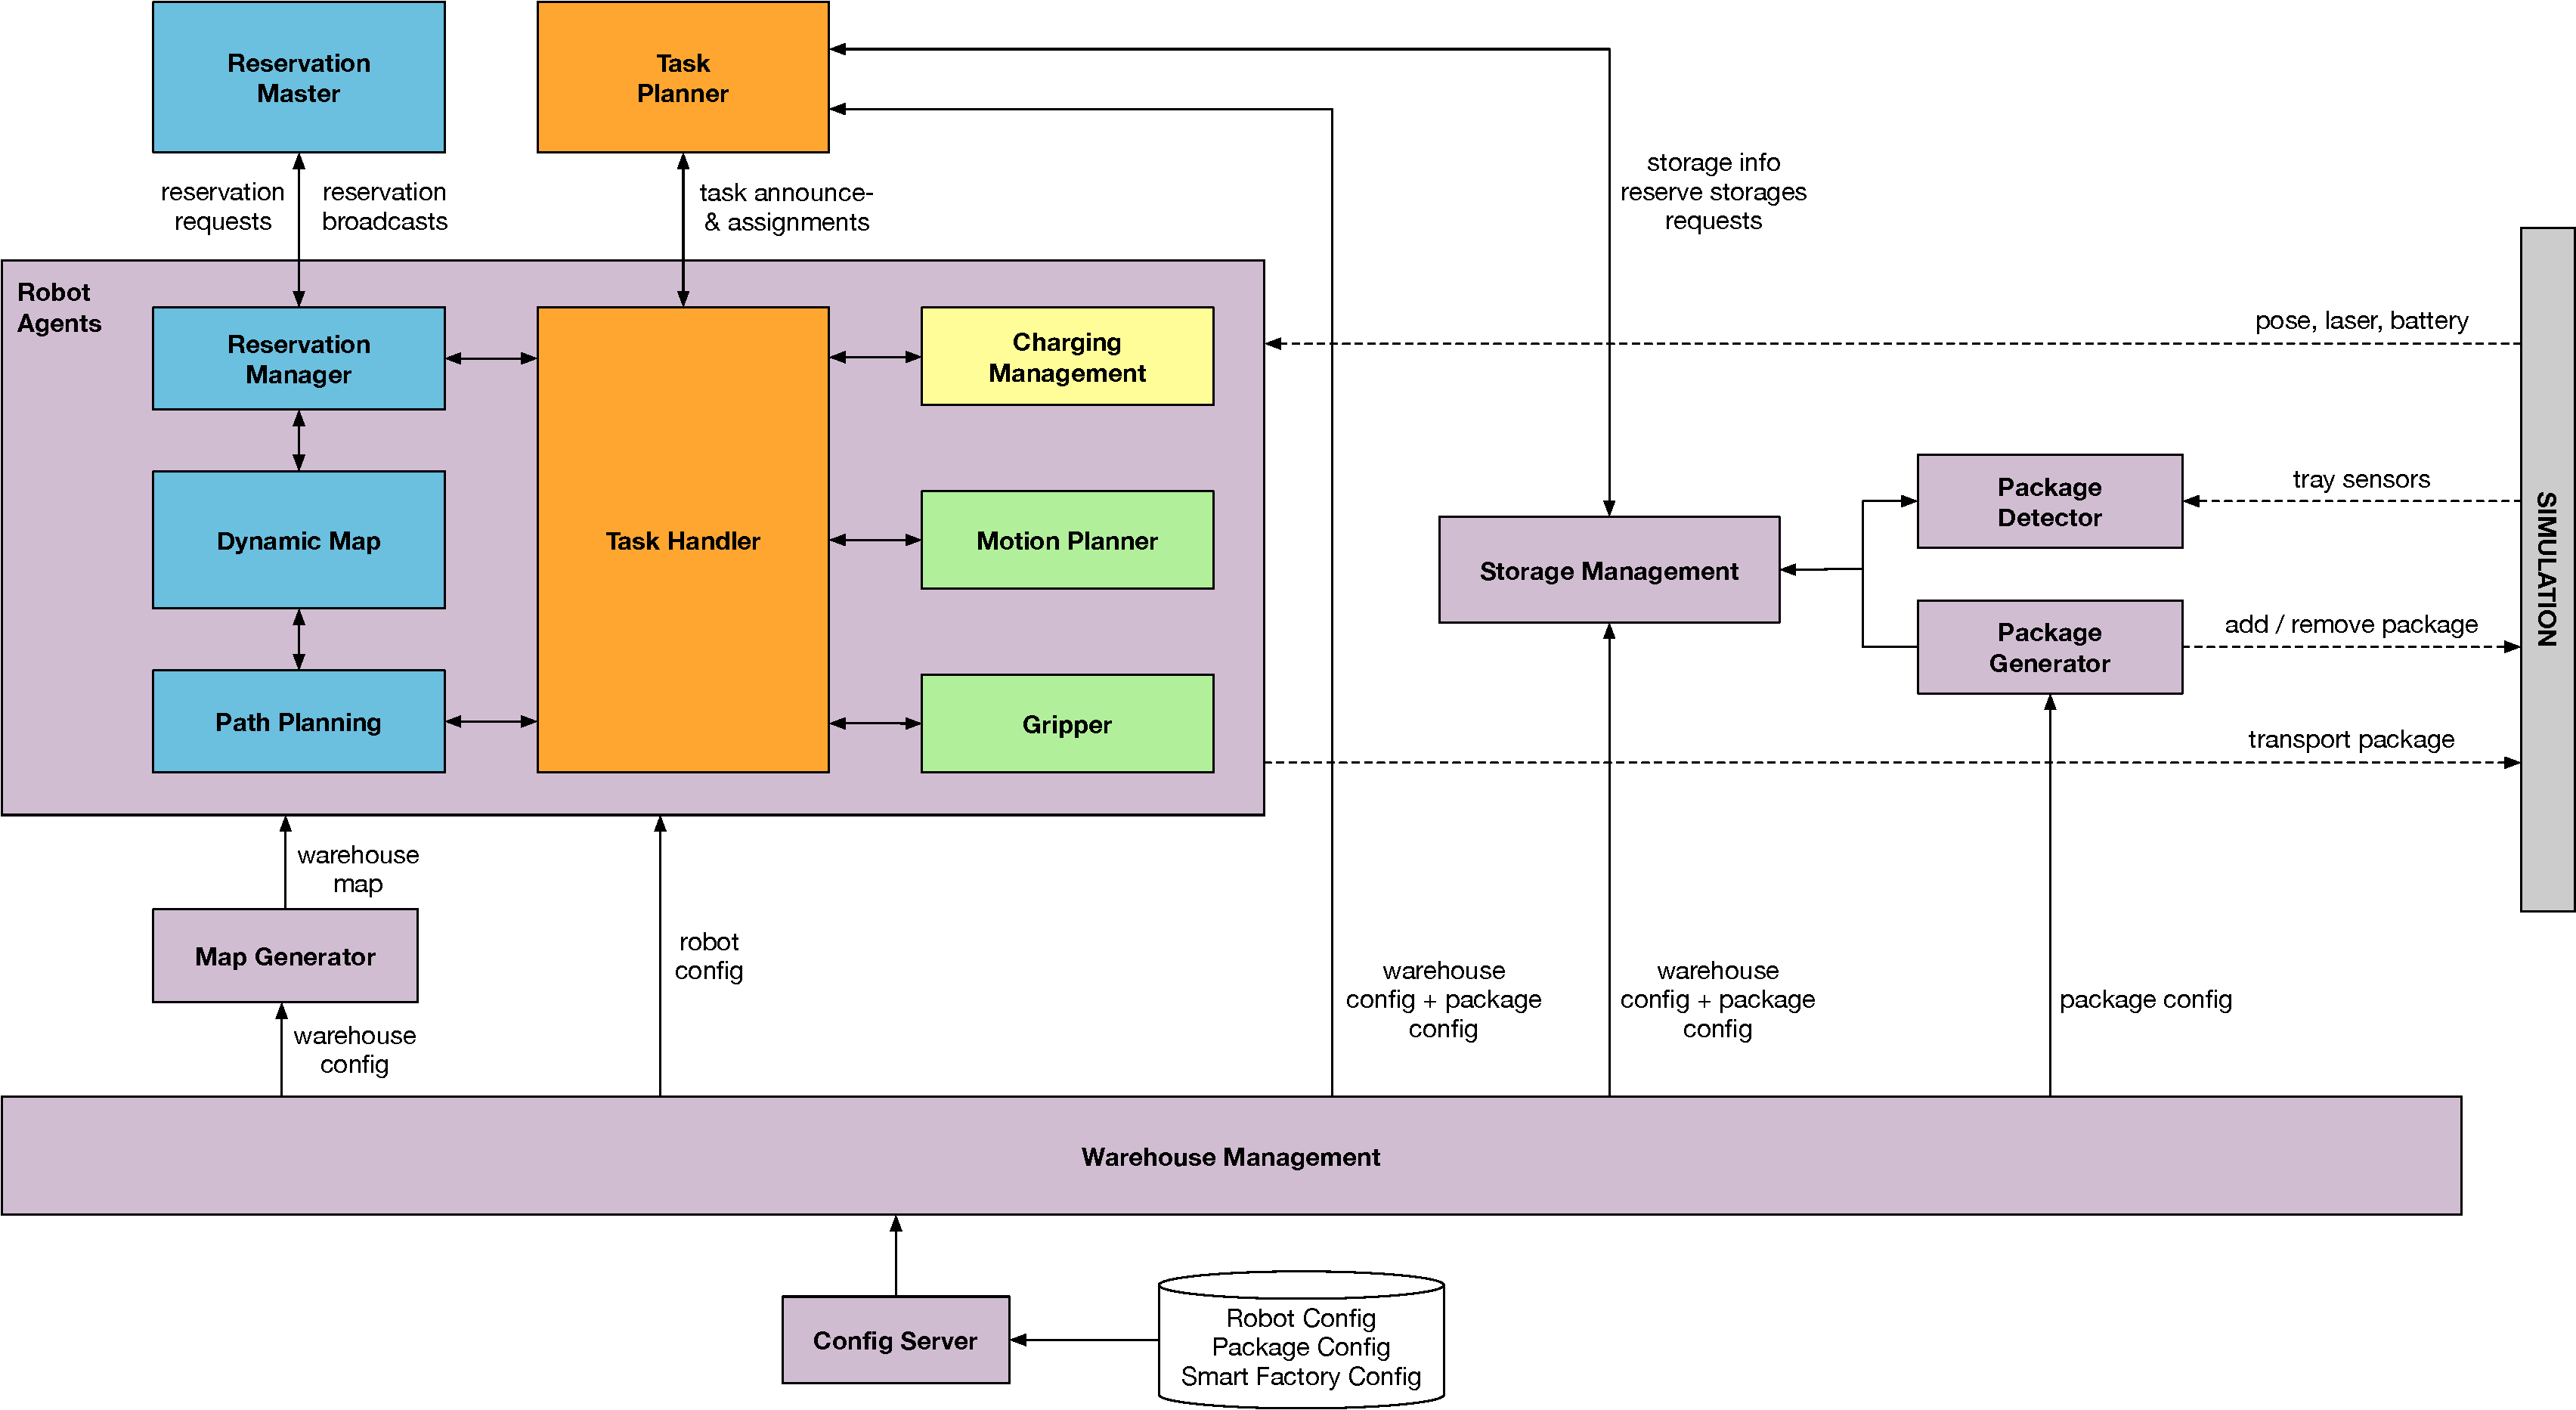
\includegraphics[width=0.45\textwidth]{resources/system_architecture}
	\caption{System Architecture}
	\label{fig:system_architecture}
\end{figure}
Test

\subsection{Task Planning}
\label{subsec:task_planning}
Describing how the task planning works.

\subsection{Path Planning}
\label{subsec:path_planning}
Describing how the path planning works. At the end of the planning the paths need to be reserved, what's described in the coordination section.

\subsection{Coordination}
\label{subsec:coordination}
Describe how the coordination between the robots work. This chapter describes the ReserverationManager and the Arbiter (and explains why we use the Arbiter).

\subsection{Motion Planning}
\label{subsec:motion_planning}
Describe how we implement the Motion Planner (PID, velocity, deceleration, departure times, ...).

\subsection{Charging Management}
\label{subsec:ChargingManagement}
Describe the role of the charging management, what it does and how it does it (e.g. penalty factor).

\subsection{Task Execution}
\label{subsec:Task Execution}
Describe how the Robot Agents operate (maybe call the section something like: Operation), how they work on the tasks, when they idle, ...

\subsection{Prototyping Environment}
\label{subsec:prototyping_environment}
Describe that we've used a prototyping environment to test all our path-planning and coordination algorithms in a simple and clean environment.

\section{Results}
\label{sec:results}
Analysing the results is a very important validation for any project. But before that, one must define exact constraints for evaluation of these results. 

\subsection{Evaluation Methodology}
\label{evaluation_methodology}
As mentioned in \ref{sec:introduction}, the goal of our system was to design a \textit{scalable} and \textit{collaborative} autonomous warehouse system. The first requirement was to able to successfully demonstrate the workability of our system. This can be separated in following sub requirements:
\begin{itemize}
\item A task should be correctly assigned to the nearest robot
\item The robot agent should complete the task by correctly following the path created by path planner.
\item The robot should be able to handle obstacles and should be able to place packages on the shelves.
\item The agent should be able to coordinate with other agents for reserving path space. 
%TODO Add more
\end{itemize}
For successful simulation: A number of robots ( \textgreater 1) must be able to handle multiple tasks. 
%TODO Add more

\subsection{Evaluation Process}
Considering all the above points, we decided to go for the following evaluation:
\\
Time required per package averaged over 40 tasks.
\begin{itemize}
\item Constant Parameters:

\begin{itemize}
\item Map: Standard
\item Starting battery: Randomized between 95 - 100%
\item Number of averaged transportation tasks: 40
\item Robot type: Default
\item Path planner: Smoothed-Theta*
\item Number of repetitions per simulation: 3
\end{itemize}

\item Variable Parameter: Number of robots
\item Evaluated Metrics:

\begin{itemize}
\item Average time required to perform task from assignment to completion
\item Average time required to perform task from execution start to completion
\item Individual time spent in:	
\begin{itemize}
\item Waiting for execution
\item Driving to pick up the package	
\item Picking up the package	
\item Driving to drop off the package	
\item Dropping off the package		

\end{itemize}

\end{itemize}

\end{itemize}

For each instance, the ROS, MORSE and RViz environment was initialized with said parameters. After 40 transportation tasks are successfully completed, a .csv file is generated with following parameters:
\begin{itemize}
\item Type of the task : If it is charging or transportation
\item ID of the robot agent  
\item ID or sequence number of the task
\item Time since start of simulation
\item Time durations for various activities like: assignment, driving to pickup, picking up, drive to dropoff and dropoff 
\end{itemize}
Then a MATLAB script converts this data into various intuitive graphs. 

%TODO Add info about graphs.

\subsection{Evaluation results and interpretation}
%TODO Show and explain results here :

Graphs and explanations
\\
FROM CAN:
\\
Think about how you can show your project’s performance. This is the most important section that will reflect your entire project, therefore it comes with the most weight on the grading of the Final Report. Therefore, analyse well what your project promises and how you can NUMERICALLY show this. Then, you discuss on the findings. Sub-sections can be created freely.
\\
Usually, the common metrics to be used are: 
\begin{itemize}
\item
overall accuracy in estimation (of whatever you are estimating: e.g. human belief, human activity, object type + shape, object pose, comparing the estimated time to store a pkg of a robot and the real time of realization etc).
Of course for such analysis you need multiple runs of the system
Don’t forget to separate the training set from the test set (80% of your entire dataset is for training, 20% is to test)

\item
overall success / precision (of the overall decisions your system makes: e.g. robotA is the most suitable for loading and storing pkg, comparison of the average time a task is realized with or without this component shows the impact of the component.)

\end{itemize}

If you can show your results on graphics it is a BONUS. If you can show on such graphs that how changing of some parameters of your mehtods/env. conditions/the context in the scenario etc. would affect your system’s performance, then you will receive +10 points for your overall document. 
\\
As the first step, you start discussing on what sort of results you will show and we will definitely discuss them in the upcoming two weeks. Feel free to suggest and ask anything on that phase (be brave !).
\\
Finally, you will conclude with the discussion of these results you showed/described. Basically answer this question, what these results tell you? Even though they are bad /not significant then you need to comment on why it is how it is. There HAS TO BE A DISCUSSION even though it is short. 
\\
You can also criticize your approach and offer better ones if it would lead to better performances. You can also briefly discuss the points to be improved/extended in your system. You will get the GRADES FROM THE DISCUSSION more than the significance or the performance of your results. In the past some groups got the highest grades although their system didn’t work well. Your goal is not to build an end product, but to be aware of what you build, a strong code base and discussion points for us to improve on your code. Positive results are of course a plus.



% needed in second column of first page if using \IEEEpubid
%\IEEEpubidadjcol

% An example of a floating figure using the graphicx package.
% Note that \label must occur AFTER (or within) \caption.
% For figures, \caption should occur after the \includegraphics.
% Note that IEEEtran v1.7 and later has special internal code that
% is designed to preserve the operation of \label within \caption
% even when the captionsoff option is in effect. However, because
% of issues like this, it may be the safest practice to put all your
% \label just after \caption rather than within \caption{}.
%
% Reminder: the "draftcls" or "draftclsnofoot", not "draft", class
% option should be used if it is desired that the figures are to be
% displayed while in draft mode.
%
%\begin{figure}[!t]
%\centering
%\includegraphics[width=2.5in]{myfigure}
% where an .eps filename suffix will be assumed under latex, 
% and a .pdf suffix will be assumed for pdflatex; or what has been declared
% via \DeclareGraphicsExtensions.
%\caption{Simulation Results}
%\label{fig_sim}
%\end{figure}

% Note that IEEE typically puts floats only at the top, even when this
% results in a large percentage of a column being occupied by floats.


% An example of a double column floating figure using two subfigures.
% (The subfig.sty package must be loaded for this to work.)
% The subfigure \label commands are set within each subfloat command, the
% \label for the overall figure must come after \caption.
% \hfil must be used as a separator to get equal spacing.
% The subfigure.sty package works much the same way, except \subfigure is
% used instead of \subfloat.
%
%\begin{figure*}[!t]
%\centerline{\subfloat[Case I]\includegraphics[width=2.5in]{subfigcase1}%
%\label{fig_first_case}}
%\hfil
%\subfloat[Case II]{\includegraphics[width=2.5in]{subfigcase2}%
%\label{fig_second_case}}}
%\caption{Simulation results}
%\label{fig_sim}
%\end{figure*}
%
% Note that often IEEE papers with subfigures do not employ subfigure
% captions (using the optional argument to \subfloat), but instead will
% reference/describe all of them (a), (b), etc., within the main caption.


% An example of a floating table. Note that, for IEEE style tables, the 
% \caption command should come BEFORE the table. Table text will default to
% \footnotesize as IEEE normally uses this smaller font for tables.
% The \label must come after \caption as always.
%
%\begin{table}[!t]
%% increase table row spacing, adjust to taste
%\renewcommand{\arraystretch}{1.3}
% if using array.sty, it might be a good idea to tweak the value of
% \extrarowheight as needed to properly center the text within the cells
%\caption{An Example of a Table}
%\label{table_example}
%\centering
%% Some packages, such as MDW tools, offer better commands for making tables
%% than the plain LaTeX2e tabular which is used here.
%\begin{tabular}{|c||c|}
%\hline
%One & Two\\
%\hline
%Three & Four\\
%\hline
%\end{tabular}
%\end{table}


% Note that IEEE does not put floats in the very first column - or typically
% anywhere on the first page for that matter. Also, in-text middle ("here")
% positioning is not used. Most IEEE journals use top floats exclusively.
% Note that, LaTeX2e, unlike IEEE journals, places footnotes above bottom
% floats. This can be corrected via the \fnbelowfloat command of the
% stfloats package.



\section{Conclusion}
FROM CAN:
\\
A brief summary of your system, what was the problem, how you achieved, your objectives, and your methodologies you used very very briefly. Then again very briefly share your finding (the discussion you made). Finally, you will conclude with the possible extensions / changes to improve the performance, basically the future works. You can find more about the templates of IEEE on the internet.




% if have a single appendix:
\appendix[Class Diagram]

Here I would like to see your final class diagram. It doesn’t require any description (unless it is complicated). It will be sufficient and necessary to mention at least once inside the methodology part that your class diagram is attached as an appendix. Also give figure caption to it.


% or
%\appendix  % for no appendix heading
% do not use \section anymore after \appendix, only \section*
% is possibly needed

% use appendices with more than one appendix
% then use \section to start each appendix
% you must declare a \section before using any
% \subsection or using \label (\appendices by itself
% starts a section numbered zero.)

% use section* for acknowledgement
\section*{Acknowledgment}


The authors would like to thank...


% Can use something like this to put references on a page
% by themselves when using endfloat and the captionsoff option.
\ifCLASSOPTIONcaptionsoff
  \newpage
\fi



% trigger a \newpage just before the given reference
% number - used to balance the columns on the last page
% adjust value as needed - may need to be readjusted if
% the document is modified later
%\IEEEtriggeratref{8}
% The "triggered" command can be changed if desired:
%\IEEEtriggercmd{\enlargethispage{-5in}}

% references section

% can use a bibliography generated by BibTeX as a .bbl file
% BibTeX documentation can be easily obtained at:
% http://www.ctan.org/tex-archive/biblio/bibtex/contrib/doc/
% The IEEEtran BibTeX style support page is at:
% http://www.michaelshell.org/tex/ieeetran/bibtex/
%\bibliographystyle{IEEEtran}
% argument is your BibTeX string definitions and bibliography database(s)
%\bibliography{IEEEabrv,../bib/paper}
%
% <OR> manually copy in the resultant .bbl file
% set second argument of \begin to the number of references
% (used to reserve space for the reference number labels box)
\begin{thebibliography}{1}

\bibitem{IEEEhowto:kopka}
H.~Kopka and P.~W. Daly, \emph{A Guide to \LaTeX}, 3rd~ed.\hskip 1em plus
  0.5em minus 0.4em\relax Harlow, England: Addison-Wesley, 1999.

\end{thebibliography}

%\vfill

% Can be used to pull up biographies so that the bottom of the last one
% is flush with the other column.
%\enlargethispage{-5in}



% that's all folks
\end{document}


